\section{Fixed-Topology Asymptotic Penalty}\label{sec:sandwich}

Under the per-instance hypothesis~\ref{prop:restricted_lower_bound}, together
with the independently proved evaluation~\ref{prop:hb-eval}, the Main Theorem
(Theorem~\ref{thm:main}) identifies the Hamming Ball as the conditional dense
limit. The following proposed sparse-limit comparison is refuted:

\begin{remark}[The proposed sparse-limit bound is false]
The proposed statement that every connected $R$-vertex subgraph $V'$ in
$A(n,k)$ is bounded above by the Star Graph $K_{1, R-1}$, yielding a total
correction $(X+D) = \binom{R}{2}$:
	\begin{equation}\label{eq:sparse-limit}
		\left| \extbd(V') \right| \le \big(R \cdot k - (R - 1)\big)(n - k) - \binom{R}{2}
	\end{equation}
The four-vertex path in $A(6,3)$ has external boundary $22$, while the
right-hand side of \eqref{eq:sparse-limit} is $21$, so the universal connected
version is false. A separate statement restricted to genuinely optimal
connected subgraphs is not refuted by this example, but is not proved here;
when a pairwise-distinct-symbol Star embeds, it gives the displayed value.
The inequality is retained only as a record of the abandoned heuristic and is
not used subsequently.
\end{remark}

\begin{figure}[H]
	\centering
	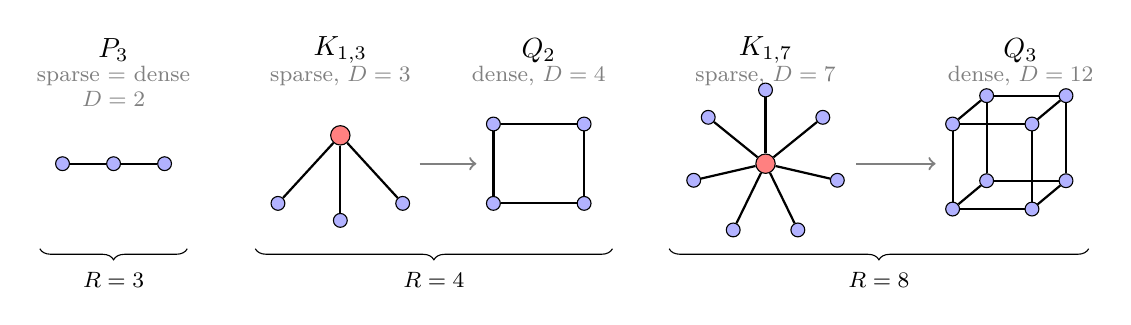
\begin{tikzpicture}[scale=0.72, font=\small,
			vertex/.style={circle, draw, fill=blue!30, inner sep=0pt, minimum size=5pt},
			hub/.style={circle, draw, fill=red!50, inner sep=0pt, minimum size=7pt}]

		% -- R=3: Path P_3 (sparse = dense) --------------------
		\node[font=\bfseries] at (0, 2.3) {$P_3$};
		\node[font=\footnotesize, text=gray] at (0, 1.85) {sparse $=$ dense};
		\node[font=\footnotesize, text=gray] at (0, 1.45) {$D=2$};

		\node[vertex] (p0) at (-0.9, 0.3) {};
		\node[vertex] (p1) at (0,    0.3) {};
		\node[vertex] (p2) at (0.9,  0.3) {};

		\draw[thick] (p0) -- (p1) -- (p2);

		% -- K_{1,3}: Star on 4 vertices -----------------------
		\node[font=\bfseries] at (4, 2.3) {$K_{1,3}$};
		\node[font=\footnotesize, text=gray] at (4, 1.85) {sparse, $D=3$};

		\node[hub]    (c1) at (4, 0.8) {};
		\node[vertex] (a1) at (2.9, -0.4) {};
		\node[vertex] (b1) at (4, -0.7) {};
		\node[vertex] (d1) at (5.1, -0.4) {};

		\draw[thick] (c1) -- (a1);
		\draw[thick] (c1) -- (b1);
		\draw[thick] (c1) -- (d1);

		% -- Q_2: Hamming Ball on 4 vertices (square) ----------
		\node[font=\bfseries] at (7.5, 2.3) {$Q_2$};
		\node[font=\footnotesize, text=gray] at (7.5, 1.85) {dense, $D=4$};

		\node[vertex] (q0) at (6.7, -0.4) {};
		\node[vertex] (q1) at (8.3, -0.4) {};
		\node[vertex] (q2) at (8.3,  1.0) {};
		\node[vertex] (q3) at (6.7,  1.0) {};

		\draw[thick] (q0) -- (q1) -- (q2) -- (q3) -- (q0);

		% Arrow between R=4 pair
		\draw[->, thick, gray] (5.4, 0.3) -- (6.4, 0.3);

		% -- K_{1,7}: Star on 8 vertices -----------------------
		\node[font=\bfseries] at (11.5, 2.3) {$K_{1,7}$};
		\node[font=\footnotesize, text=gray] at (11.5, 1.85) {sparse, $D=7$};

		\node[hub] (c2) at (11.5, 0.3) {};
		\foreach \i/\a in {1/90,2/141,3/193,4/244,5/296,6/347,7/39} {%
				\node[vertex] (s\i) at ({11.5 + 1.3*cos(\a)}, {0.3 + 1.3*sin(\a)}) {};
				\draw[thick] (c2) -- (s\i);
			}

		% -- Q_3: Hamming Ball on 8 vertices (cube) ------------
		\node[font=\bfseries] at (16, 2.3) {$Q_3$};
		\node[font=\footnotesize, text=gray] at (16, 1.85) {dense, $D=12$};

		% Front face
		\node[vertex] (f0) at (14.8, -0.5) {};
		\node[vertex] (f1) at (16.2, -0.5) {};
		\node[vertex] (f2) at (16.2,  1.0) {};
		\node[vertex] (f3) at (14.8,  1.0) {};
		% Back face (offset)
		\node[vertex] (b0) at (15.4,  0.0) {};
		\node[vertex] (b1a) at (16.8,  0.0) {};
		\node[vertex] (b2) at (16.8,  1.5) {};
		\node[vertex] (b3) at (15.4,  1.5) {};

		% Front edges
		\draw[thick] (f0) -- (f1) -- (f2) -- (f3) -- (f0);
		% Back edges
		\draw[thick] (b0) -- (b1a) -- (b2) -- (b3) -- (b0);
		% Connecting edges
		\draw[thick] (f0) -- (b0);
		\draw[thick] (f1) -- (b1a);
		\draw[thick] (f2) -- (b2);
		\draw[thick] (f3) -- (b3);

		% Arrow between R=8 pair
		\draw[->, thick, gray] (13.1, 0.3) -- (14.5, 0.3);

		% R=3 brace
		\draw[decorate, decoration={brace, mirror, amplitude=4pt}] (-1.3, -1.2) -- (1.3, -1.2)
		node[midway, below=5pt, font=\footnotesize] {$R = 3$};
		% R=4 brace
		\draw[decorate, decoration={brace, mirror, amplitude=4pt}] (2.5, -1.2) -- (8.8, -1.2)
		node[midway, below=5pt, font=\footnotesize] {$R = 4$};
		% R=8 brace
		\draw[decorate, decoration={brace, mirror, amplitude=4pt}] (9.8, -1.2) -- (17.2, -1.2)
		node[midway, below=5pt, font=\footnotesize] {$R = 8$};
	\end{tikzpicture}
	\caption{Sparse and dense limits. At $R=3$ the star graph and Hamming Ball
	coincide (both are $P_3$). At $R=4$ the gap is 1 defect link; at $R=8$ it
	widens to 5. Arrows connect the sparse limit $K_{1,R-1}$ ($D = R - 1$) to
	the dense limit $Q_d$ ($D = \Eseq(R)$).}
	\label{fig:limits}
\end{figure}

\paragraph{Structural Convergence at $R=3$.}
Our explicit bounds coincide structurally at exactly $R=3$. For the Dense Limit
(Hamming Ball), we have $\Eseq(3) = 2$ and $\Cconst(3) = 3$. For the Sparse
Limit (Star Graph), a $K_{1,2}$ structure yields defect $D = 2$,
cross-collisions $X=1$, and a total correction $(X + D) = \binom{3}{2} = 3$. The
As abstract graphs, both configurations are a three-vertex path, but their
embedded root incidences need not agree; in particular, $X$ is not determined
by the abstract graph. This records an abstract-topology coincidence, not
uniqueness of embedded extremizers.

\begin{theorem}[Fixed-Topology Asymptotic Penalty]\label{thm:penalty}
Fix a connected topology (isomorphism type) on $R$ vertices, embedded as
$V'_{\mathrm{sub}} \subseteq V(A(n,k))$, with defect shortfall $\Delta D =
\Eseq(R) - D(V'_{\mathrm{sub}}) > 0$ relative to the Hamming Ball
$V'_{\mathrm{opt}} = \mathrm{HB}_R$. Then
	\begin{equation}\label{eq:penalty-asymptotic}
		\left| \extbd(V'_{\mathrm{sub}}) \right| - \left| \extbd(V'_{\mathrm{opt}}) \right| = \Delta D \cdot (n-k) + O_R(1),
	\end{equation}
where the $O_R(1)$ term depends only on the fixed embedded configuration (not
on $n$ or $k$ once that configuration is realizable).
Consequently, for every fixed sub-optimal topology there is a threshold
$(n-k)_0$, depending only on that topology, beyond which $\left|
\extbd(V'_{\mathrm{sub}}) \right| > \left| \extbd(V'_{\mathrm{opt}}) \right|$.
\end{theorem}
To understand this mechanism, we return to the exact boundary
decomposition~\eqref{eq:boundary}:

Recall that the defect is defined as $D(V') = |V'| \cdot k - U(V')$. If a subset
$V'$ falls short of the optimal Hamming Ball defect by $\Delta D$, it must
project onto $\Delta D$ \emph{additional} unique roots to maintain its vertex
count ($U_{\mathrm{sub}} = U_{\mathrm{opt}} + \Delta D$).

Substituting this into the boundary equation yields the comparative boundary
size:
\begin{align}\label{eq:penalty-expansion}
	\left| \extbd(V'_{\mathrm{sub}}) \right| & = (U_{\mathrm{opt}} + \Delta D) \cdot (n - k) - (X_{\mathrm{sub}} + D_{\mathrm{sub}}) \nonumber                                                     \\
	                                         & = \left| \extbd(V'_{\mathrm{opt}}) \right| + \Delta D \cdot (n - k) + (X_{\mathrm{opt}} + D_{\mathrm{opt}}) - (X_{\mathrm{sub}} + D_{\mathrm{sub}})
\end{align}

This formulation isolates the asymptotic behavior. The correction term
$(X_{\mathrm{opt}} + D_{\mathrm{opt}}) - (X_{\mathrm{sub}} + D_{\mathrm{sub}})$
is a genuine constant for a fixed embedded configuration: $X$ and $D$ do not
depend on the ambient dimensions
$n, k$ once they are large enough to realize it (the same dimension-independence
exploited in the verification engine, Appendix~\ref{app:engine}). We emphasize
that we do \emph{not} claim this correction is always non-negative --- the exact
sign and magnitude vary by topology, and no dimension-independent bound of the
form $X(V')+D(V') \le f(R)$ has been established for arbitrary connected
topologies (indeed, an earlier, stronger candidate bound was refuted by an
explicit counterexample; see the discussion accompanying
Proposition~\ref{prop:restricted_lower_bound}). What is unconditionally true is only that the
correction is \emph{fixed} while $\Delta D \cdot (n-k)$ grows linearly in
$(n-k)$: for $\Delta D \ge 1$, the linear term eventually dominates any fixed
constant, however large, as $(n-k) \to \infty$. This is the precise and provable
content of the Fixed-Topology Asymptotic Penalty: it guarantees eventual, not
immediate, dominance of the Hamming Ball, with the crossover point depending on
the specific sub-optimal topology.

\subsection{Numerical Illustration}

To visualize the Fixed-Topology Asymptotic Penalty, we walk through \emph{every}
achievable defect value for connected $8$-vertex subgraphs in $A(n,k)$, where
$n$ and $k$ are the graph parameters from Definition~2.2. The Hamming Ball
($Q_3$) achieves $D = 12$; the fracture gap (Theorem~\ref{thm:fracture}) forbids
$D = 11$; and the Continuity construction (Theorem~\ref{thm:continuity}) fills
in every integer from $10$ down to $7$. The full achievable spectrum is $\{7,\,
8,\, 9,\, 10,\, 12\}$.

\begin{table}[ht]
	\centering
	\caption{Complete defect walk-through for $R=8$ in $A(n,k)$, valid for any
	$k \ge 3$.  Each row is verified by exhaustive search over all connected
	$8$-vertex subgraphs.}
	\label{tab:walkthrough_r8}
	\begin{tabular}{@{}clcl@{}}
		\toprule
		$D(V')$   & Construction                    & $U$       & Boundary                \\
		\midrule
		12        & $Q_3$ (Hamming Ball)            & $8k{-}12$ & $(8k{-}12)(n{-}k) - 12$ \\
		\emph{11} & \emph{forbidden (fracture gap)} & ---       & ---                     \\
		10        & $Q_3 - v + \text{leaf}$         & $8k{-}10$ & $(8k{-}10)(n{-}k) - 16$ \\
		9         & partial connection              & $8k{-}9$  & $(8k{-}9)(n{-}k) - 18$  \\
		8         & partial connection              & $8k{-}8$  & $(8k{-}8)(n{-}k) - 22$  \\
		7         & $K_{1,7}$ (Star Graph)          & $8k{-}7$  & $(8k{-}7)(n{-}k) - 28$  \\
		\bottomrule
	\end{tabular}
\end{table}

\noindent Each missing defect link increases $U$ by one, adding $(n{-}k)$ to the
boundary. The total correction constants ($12, 16, 18, 22, 28$) are fixed by the
graph structure and bounded by $\binom{8}{2} = 28$; as $n \to \infty$, the
boundary ranking is determined entirely by $D(V')$.

\paragraph{Convergence Near Powers of 2 ($R=7$ vs $R=8$):}
The dominance of the Hamming Ball fluctuates based on how closely $R$ fits a
perfect hypercube embedding. At $R=7$, the gap between the optimal ($D=9$) and
the 2nd best ($D=8$) is only $1(n-k)$, whereas at $R=8$, the gap jumps to
$2(n-k)$ because $D=11$ is unrealizable (Theorem~\ref{thm:fracture}). At powers
of 2, the optimal solution becomes increasingly stable relative to its nearest
competitors as the network dimensions scale.

\begin{table}[ht]
	\centering
	\caption{Defect gap between $R=7$ and $R=8$.}
	\label{tab:gap_jump}
	\begin{tabular}{@{}lccc@{}}
		\toprule
		Cluster Size $R$ & Optimal $D$ & 2nd Best $D$ & Gap ($\Delta D$) \\
		\midrule
		7 (Near-Cube)    & 9           & 8            & 1                \\
		8 (Perfect Cube) & 12          & 10           & 2                \\
		9 (Over-Cube)    & 13          & 12           & 1                \\
		\bottomrule
	\end{tabular}
\end{table}

The numerical results give fixed-topology comparisons at $n=100$.  The margin
of $464$ uses $k=4$, while the margin of $190$ uses $k=3$; they are not two
competitors in one common parameter cell.  At the common choice $k=7$, the
corresponding margins are $449$ and $182$.  These are fixed-topology
comparisons, not proofs that the Hamming Ball is the unique minimizer.

\paragraph{The Structural Inversion: Hypercubes vs.\ Arrangement Graphs.}
Comparisons with hypercube variants such as Augmented Cubes
\cite{cheng2023augmented} motivate examining Star Graphs as a competing
construction, but this paper does not establish a universal Star optimum in
either model.  The exact arrangement-graph mechanism is instead the
fixed-topology penalty: missing defect contributes a term linear in $n-k$,
while the Star produces cross-collisions that
scale quadratically as $\binom{R-1}{2}$, quickly overpowering the static penalty
and minimizing the boundary. In $A(n,k)$, however, the penalty for each missing
unit of defect is $(n-k)$ (Theorem~\ref{thm:penalty}). Because $(n-k)$ scales
with the network dimensions, it eventually dominates the static savings of a
fixed Star topology. Thus the argument establishes eventual fixed-topology
dominance only; it does not prove a permanent global inversion over all
topologies and parameter ranges.
